%%%%%%%%%%%%%%%%%%%%%%%%%%%%%%%%%%%%%%%%%
% Stylish Article
% LaTeX Template
% Version 2.1 (1/10/15)
%
% This template has been downloaded from:
% http://www.LaTeXTemplates.com
%
% Original author:
% Mathias Legrand (legrand.mathias@gmail.com) 
% With extensive modifications by:
% Vel (vel@latextemplates.com)
%
% License:
% CC BY-NC-SA 3.0 (http://creativecommons.org/licenses/by-nc-sa/3.0/)
%
%%%%%%%%%%%%%%%%%%%%%%%%%%%%%%%%%%%%%%%%%

%----------------------------------------------------------------------------------------
%	PACKAGES AND OTHER DOCUMENT CONFIGURATIONS
%----------------------------------------------------------------------------------------

\documentclass[fleqn,12pt]{SelfArx} % Document font size and equations flushed left

\usepackage[english]{babel} % Specify a different language here - english by default

\usepackage{lipsum} % Required to insert dummy text. To be removed otherwise

%----------------------------------------------------------------------------------------
%	COLUMNS
%----------------------------------------------------------------------------------------

\setlength{\columnsep}{0.55cm} % Distance between the two columns of text
\setlength{\fboxrule}{0.75pt} % Width of the border around the abstract

%----------------------------------------------------------------------------------------
%	COLORS
%----------------------------------------------------------------------------------------

\definecolor{color1}{RGB}{0,0,90} % Color of the article title and sections
\definecolor{color2}{RGB}{0,20,20} % Color of the boxes behind the abstract and headings

%----------------------------------------------------------------------------------------
%	HYPERLINKS
%----------------------------------------------------------------------------------------

\usepackage{hyperref} % Required for hyperlinks
\hypersetup{hidelinks,colorlinks,breaklinks=true,urlcolor=color2,citecolor=color1,linkcolor=color1,bookmarksopen=false,pdftitle={Title},pdfauthor={Author}}

%----------------------------------------------------------------------------------------
%	ARTICLE INFORMATION
%----------------------------------------------------------------------------------------

\JournalInfo{6.867 Final Paper} % Journal information
\Archive{} % Additional notes (e.g. copyright, DOI, review/research article)

\PaperTitle{How Does Content Drive Viewership?} % Article title

\Authors{Dave Holtz\textsuperscript{1}, Jeremy Yang\textsuperscript{2}, Michael Zhao\textsuperscript{3}} % Authors
\affiliation{\textsuperscript{1}\textit{dholtz@mit.edu}}
\affiliation{\textsuperscript{2}\textit{zheny@mit.edu}} 
\affiliation{\textsuperscript{3}\textit{mfzhao@mit.edu}}

\Keywords{} % Keywords - if you don't want any simply remove all the text between the curly brackets
\newcommand{\keywordname}{Keywords} % Defines the keywords heading name

%----------------------------------------------------------------------------------------
%	ABSTRACT
%----------------------------------------------------------------------------------------

\Abstract{Why do some webpages receive massive numbers of page views? To determine how content drives viewership, we construct a unique dataset of all articles published by the New York Times (NYT) in August 2013. Our dataset is built from 2 major components, the NYT's internal web traffic data and article content data parsed from the NYT website. We use the internal web traffic data to accurately track the number of page views of each article as well as construct a set of robust control variables such as the desk and section of each article. To build content features, we use various machine learning and statistical natural language processing techniques on our parsed article content data and construct features such as article perplexity, sentiment, reading difficulty, and indicators that denote the presence of pictures, videos, etc. Additionally, we have access to the NYT's internal website traffic data. We feed all of our constructed features to into a predictive regression model. We find [MAJOR RESULTS HERE].
}

%----------------------------------------------------------------------------------------

\begin{document}

\flushbottom % Makes all text pages the same height

\maketitle % Print the title and abstract box

\tableofcontents % Print the contents section

\thispagestyle{empty} % Removes page numbering from the first page

%----------------------------------------------------------------------------------------
%	ARTICLE CONTENTS
%----------------------------------------------------------------------------------------

\section{Introduction} % The \section*{} command stops section numbering

In today's digital economy, many companies are very interested in attracting users to visit their websites in order to earn ad revenue. While many factors might motivate a user to visit a particular page, certainly one important factor is the content in that webpage. This paper explores the relationship between the content of a webpage and the number of page views it ultimately ends up receiving by constructing a unique dataset of all articles published by the New York Times (NYT) during August 2013. This dataset is built from two major components: the NYT's internal web traffic data and parsed NYT article content data.

Typically, a study such as ours tends to be very difficult to conduct as either accurate measures of viewership are unavailable\footnote{While oftentimes precise viewership data tends to be not available openly, oftentimes researchers use related observables, such as Facebook likes} or the feature extraction of the content is too challenging (for example Youtube), or or both. Fortunately, our access to the the NYT's internal web traffic data allows us to exactly measure the number of page views an article receives. The web traffic data is rather rich and also includes internal meta-data that we use to build various control features. Moreover, since we are working with mostly textual data, we are able to take advantage of recent advancements in machine learning and statistical NLP to do feature extraction on article text. 

A similar study by Berger and Milkman (2012) \cite{berger2012makes} examines the relationship between content and word-of-mouth virality. They find that the emotional content of a NYT article is predictive of its virality. Using simple measures of an article's sentiment and emotionality, Berger and Milkman show that positive articles are more likely to show up on the New York Times "Most-Emailed" list. They also show that articles that evoke high physiological positive or negative arousal (such as awe or anger) tend to be more viral than articles that evoke deactivating emotions (sadness). We build on this study in two ways: first, we relate an article's content back to the number of page views it receives rather than its virality\footnote{Which companies arguably care more about since word-of-mouth virality is usually a means to increase page views}. Second, we employ more sophisticated machine learning feature extraction techniques to see if they work any better over their simple measures.
%------------------------------------------------

\section{Data}
\subsection{NYT Internal Web Traffic Data}
Our NYT internal web traffic dataset is a record of all individual user activity on the NYT website covering the period of April 3rd, 2013 to October 31st, 2013. This activity data is stored as individual lines of json and includes who (if available) accessed what page at what time. Overall, it is over 20 terabytes in size and contains over 3 billion page views\footnote{Not all page views are content views, for example, some events that are also tracked are searches, or user account settings.} Since the scope of this dataset is so large, we initially restrict this project to a single month, August 2013. 

We limit our dataset to consist of pages that only contain articles or blogposts published during the month of August. We parse the data to obtain a list of urls, which need to be stripped of potential garbage. After cleaning up the url data, we are left with 6682 unique pieces of content. We then parse our dataset and aggregate the number of counts each url receives. In order to make the comparison between articles fairer since an article that's been out longer will have more page views on average, we only count the number of page views received up to 7 days after publication\footnote{Given that page views tend to sharply drop off soon after publication since recency is quite important to the News, the number of page views obtained during the 7 days after an article is published represents the vast majority (usually well over 90\%) of total page views an article receives.}. In total, our data consists of over 250 million page views. As seen in Figure 1 below, the distribution of page views is highly skewed with very heavy tails. After applying a log transformation (as seen in Figure 2), our distribution looks considerably more normal. 

\begin{figure}[ht]\centering
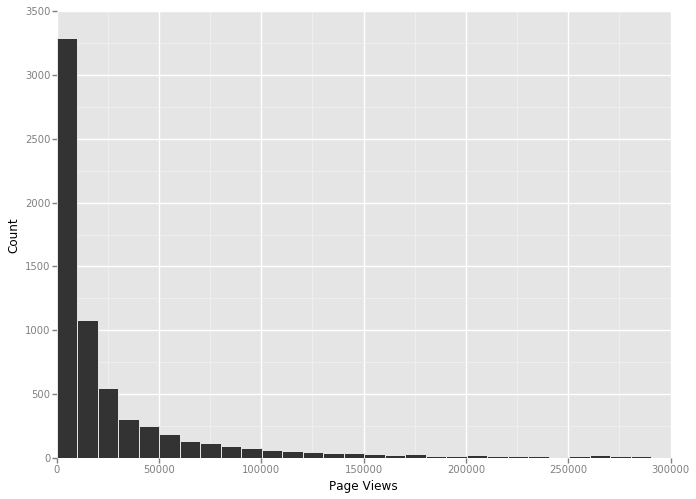
\includegraphics[width=\linewidth]{pageviews_hist}
\caption{Histogram of Articles by Number of Page Views}
\label{fig:pv_hist}
\end{figure}
% TWEAK TABLE LOOK
\begin{table}[hbt]
\caption{Page Views Distribution Summary Statistics}
\centering
\begin{tabular}{rr}
\toprule
Total Page Views  &  248161455\\
\midrule
Min               &  1\\
Max               &  2545288\\  
Mean              &  37138.8\\
Median            &  10298.5\\
Std. Dev.         &  88972.9\\
Skewness          &  9.52191\\
Kurtosis          &  173.061\\
\midrule
Observations &  6682\\
\bottomrule
\end{tabular}
\end{table}

\begin{figure}[ht]\centering
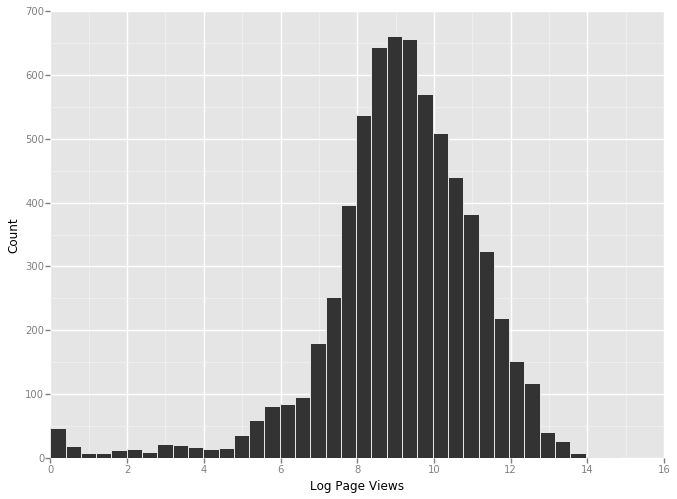
\includegraphics[width=\linewidth]{log_pageviews_hist}
\caption{Histogram of Articles by Log of Page Views}
\label{fig:lpv_hist}
\end{figure}

\begin{table}[hbt]
\caption{Log Page Views Distribution Summary Statistics}
\centering
\begin{tabular}{rr}
\toprule
Min               &  0\\
Max               &  14.74975\\  
Mean              &  9.122868\\
Median            &  9.239754\\
Std. Dev.         &  2.028668\\
Skewness          &  -1.270368\\
Kurtosis          &  3.800911\\
\midrule
Observations &  6682\\
\bottomrule
\end{tabular}
\end{table}


In addition to aggregating the counts, when 

\subsection{Parsed NYT Article Content Data}

\begin{figure}[ht]\centering
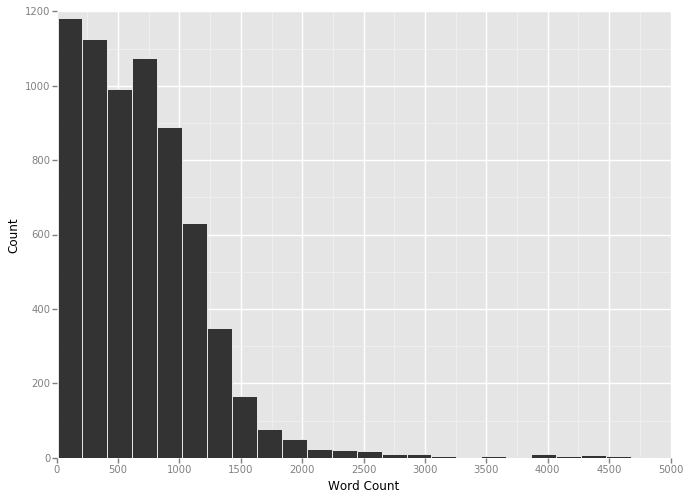
\includegraphics[width=\linewidth]{wordcount_hist}
\caption{Histogram of Articles by Word Count}
\label{fig:pv_hist}
\end{figure}

\begin{figure}[ht]\centering
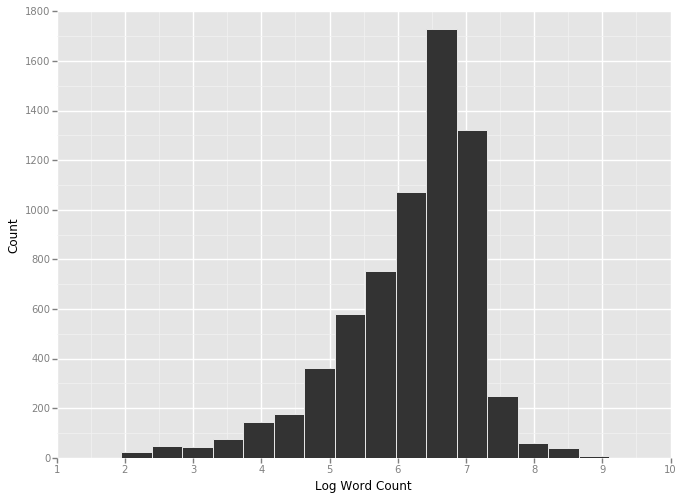
\includegraphics[width=\linewidth]{log_wordcount_hist}
\caption{Histogram of Articles by Log Word Count}
\label{fig:lpv_hist}
\end{figure}

%\begin{figure*}[ht]\centering % Using \begin{figure*} makes the figure take up the entire width of the page
%\includegraphics[width=\linewidth]{view}
%\caption{Wide Picture}
%\label{fig:view}
%\end{figure*}

%------------------------------------------------

\section{Constructed Features}

In preparing to perform our regression, we construct a number of features, using both the parsed NYT article data and secondary sources. These features include the Flesch reading ease, the (guessed) gender of the author(s), the popularity of the author(s), the sentiment of the article text, the perplexity of the article text, and variables indicating the section the article appeared in and the article's content type. Found below is a full list of these features, as well as the methodology used to construct them and validation of the features, where appropriate.

\begin{description}
	\item[Flesch Reading Ease] The Flesch reading ease is a metric developed by Flesch in 1948 \cite{flesch1948new}. The score indicates how difficult a piece of English text is to understand. Lower scores correspond to more difficult passages, and the highest score attainable is 120.0. The formula for calculating a passage's Flesch reading ease is
	
	\begin{equation}
	206.835 - 1.015 \left ( \frac{\textrm{\# words}}{\textrm{\# sentences}} \right ) - 84.6 \left ( \frac{\textrm{\# syllables}}{\textrm{\# words}} \right )
	\end{equation}
	
	To calculate the Flesch reading ease, we use the python library ``textstat." Despite the fact that the above formula is relatively straightforward, the task of counting the number of syllables in a block of text is non-trivial, so we rely on ``textstat" to do so accurately. In cases where the Flesch reading ease was for some reason null (e.g., a blog post containing only a picture), we assign the Flesch reading ease its median value.
	
	\item[Author Popularity] We attempt to include some measure of a particular author's popularity. It stands to reason that a new article by Paul Krugman or A.O. Scott should garner more readership than a new article by an unknown graduate student enrolled in 6.867 at MIT! 
	
	In order to measure something that will serve as a decent proxy for popularity, we programmatically searched for every distinct author in our dataset using Bing, and recorded the number of search results that were returned by the query. In cases where a particular article has more than one distinct author, we calculate an ``effective" popularity by simply calculating the average number of search results over all article authors.
	
	\item[Author Gender] We also attempt to construct a feature that indicates the most likely gender of the article author(s). In cases where the gender of the author is unclear (e.g., Robin) or there are likely multiple authors with different genders (e.g., The New York Times Staff), we record a third gender value, ``ambiguous / unknown." 
	
	We construct our gender data by cross-referencing the first names of all of the authors in our dataset against U.S. Social Security Administration baby name data from 1935 to 1997. If over 90\% of the babies with a given name have been male, we assume a given author is male. If over 90\% of the babies with a given name have been female, we assume a given author is female. Otherwise, we record ``ambiguous / unknown."
	
	\item[Material Type, Section, Desk, and Article Type] We also include dummy variables including the material type (e.g., `News' or `Obituary'), desk (e.g., `Weekend' or `Real Estate'), article type (`Blog post' or `Article'), and section (e.g., `Movies' or `World').

\begin{figure}[ht]\centering
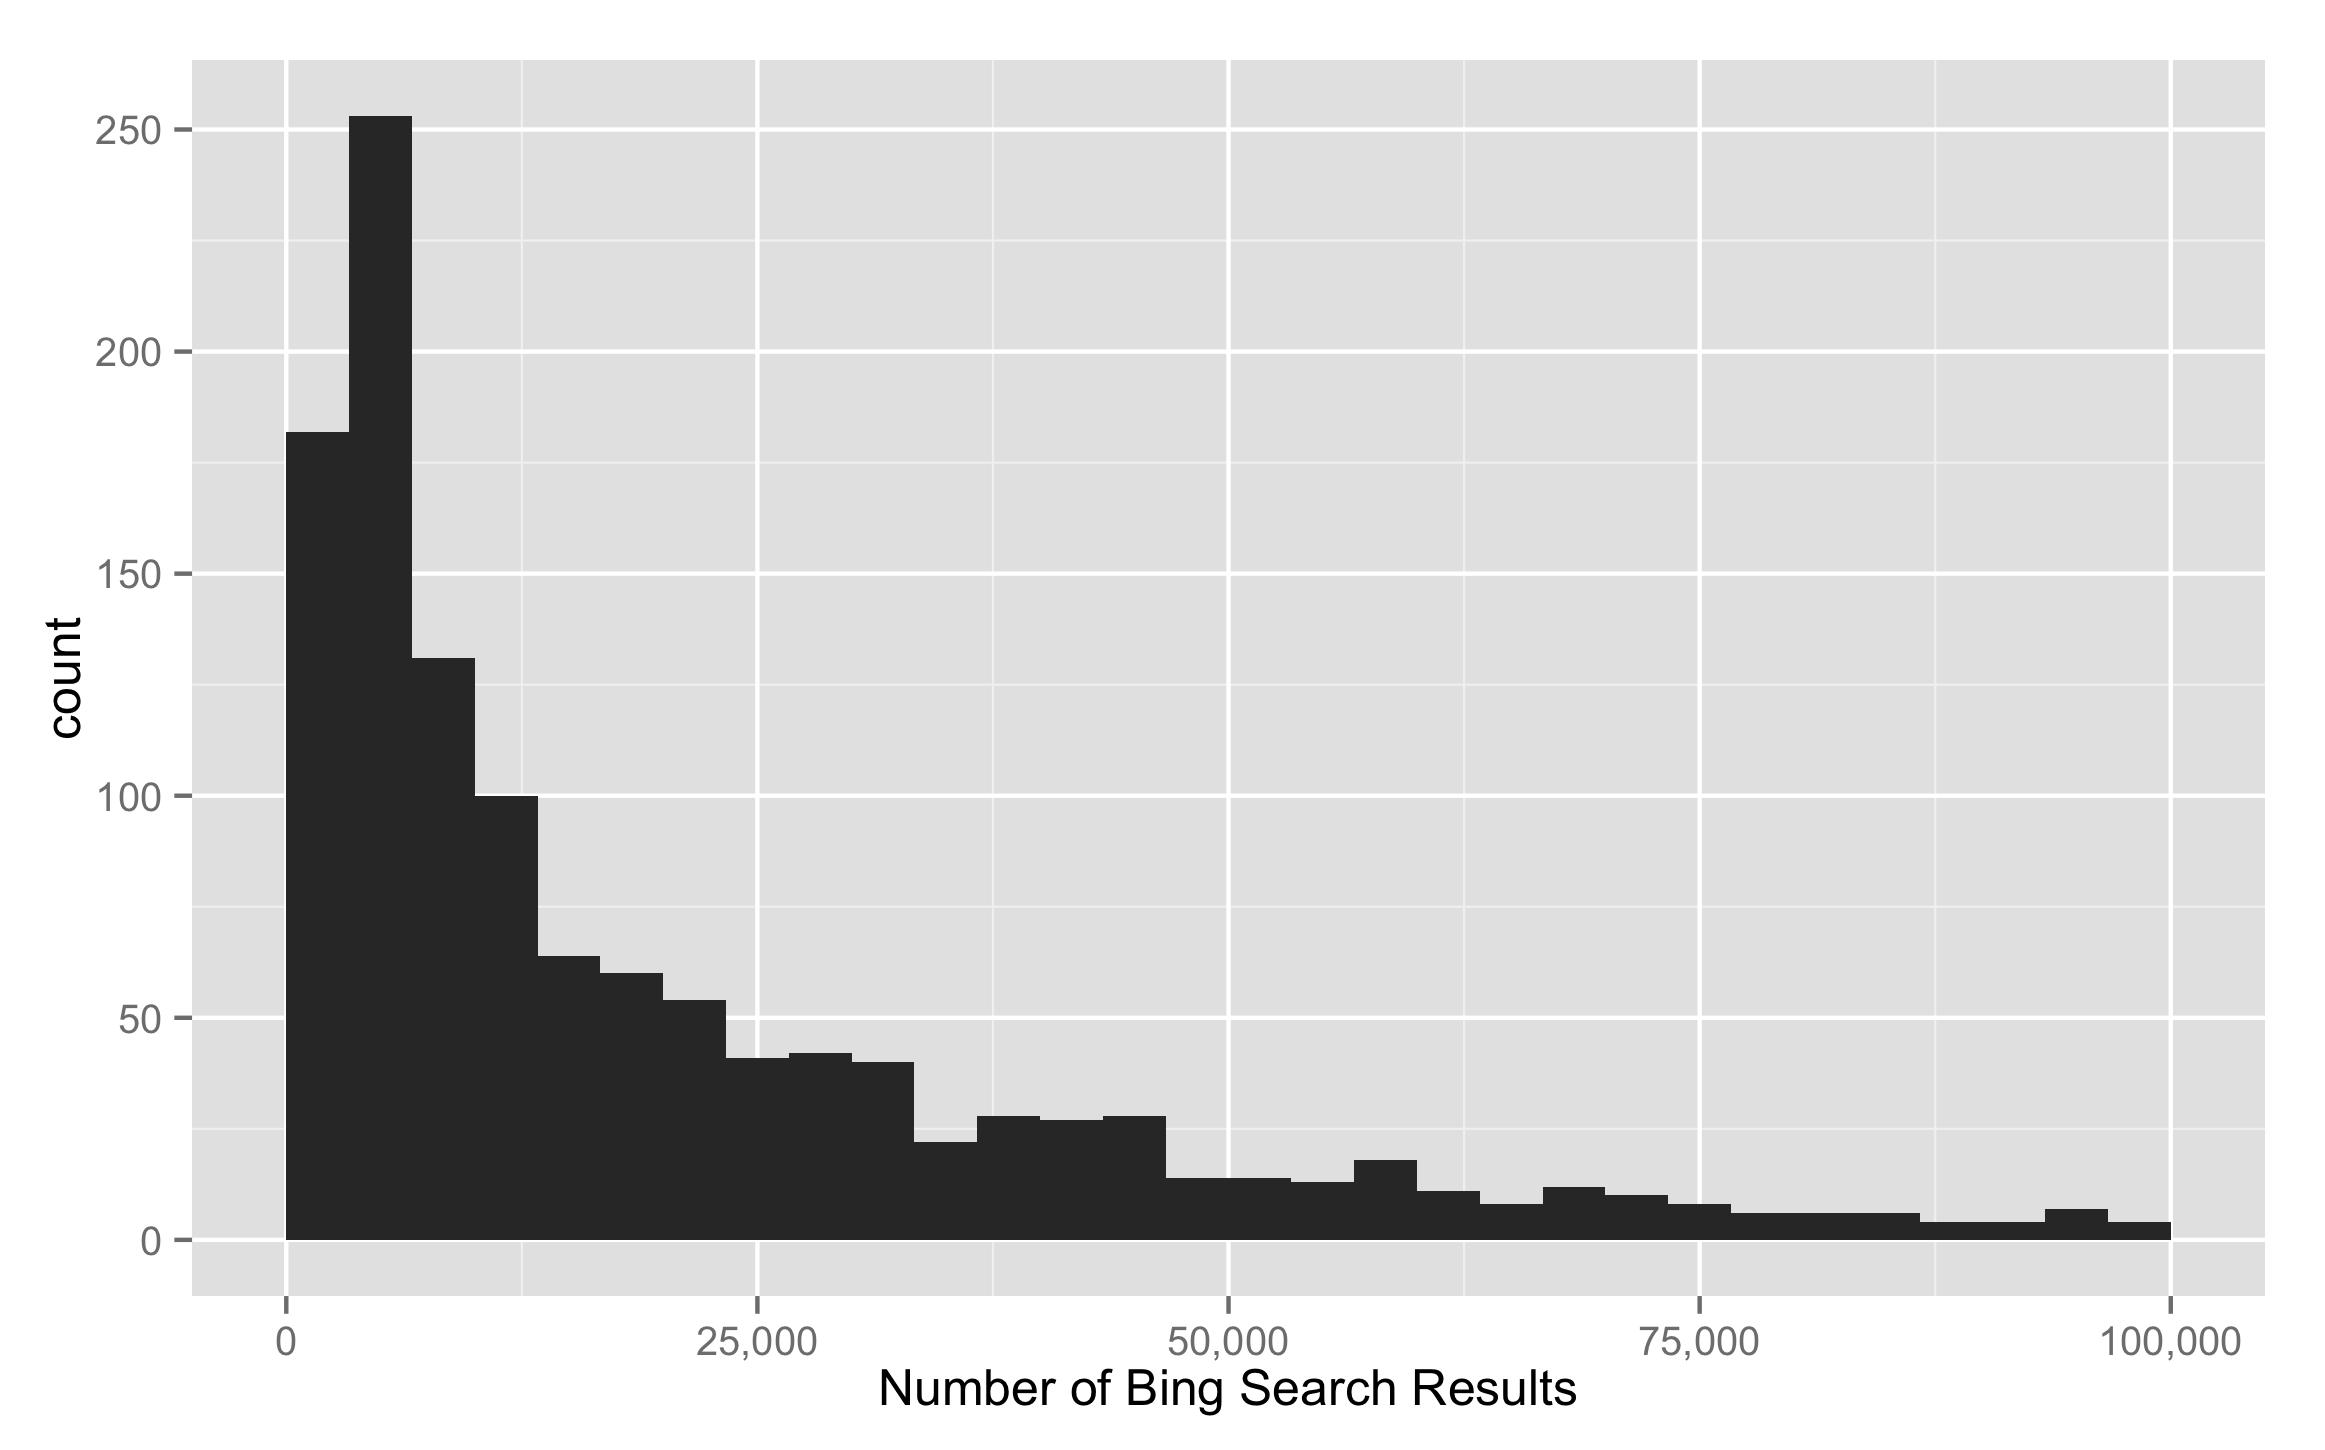
\includegraphics[width=\linewidth]{author_popularity_histogram.png}
\caption{Histogram of Bing Search Results}
\label{fig:ap_hist}
\end{figure}

\begin{figure}[ht]\centering
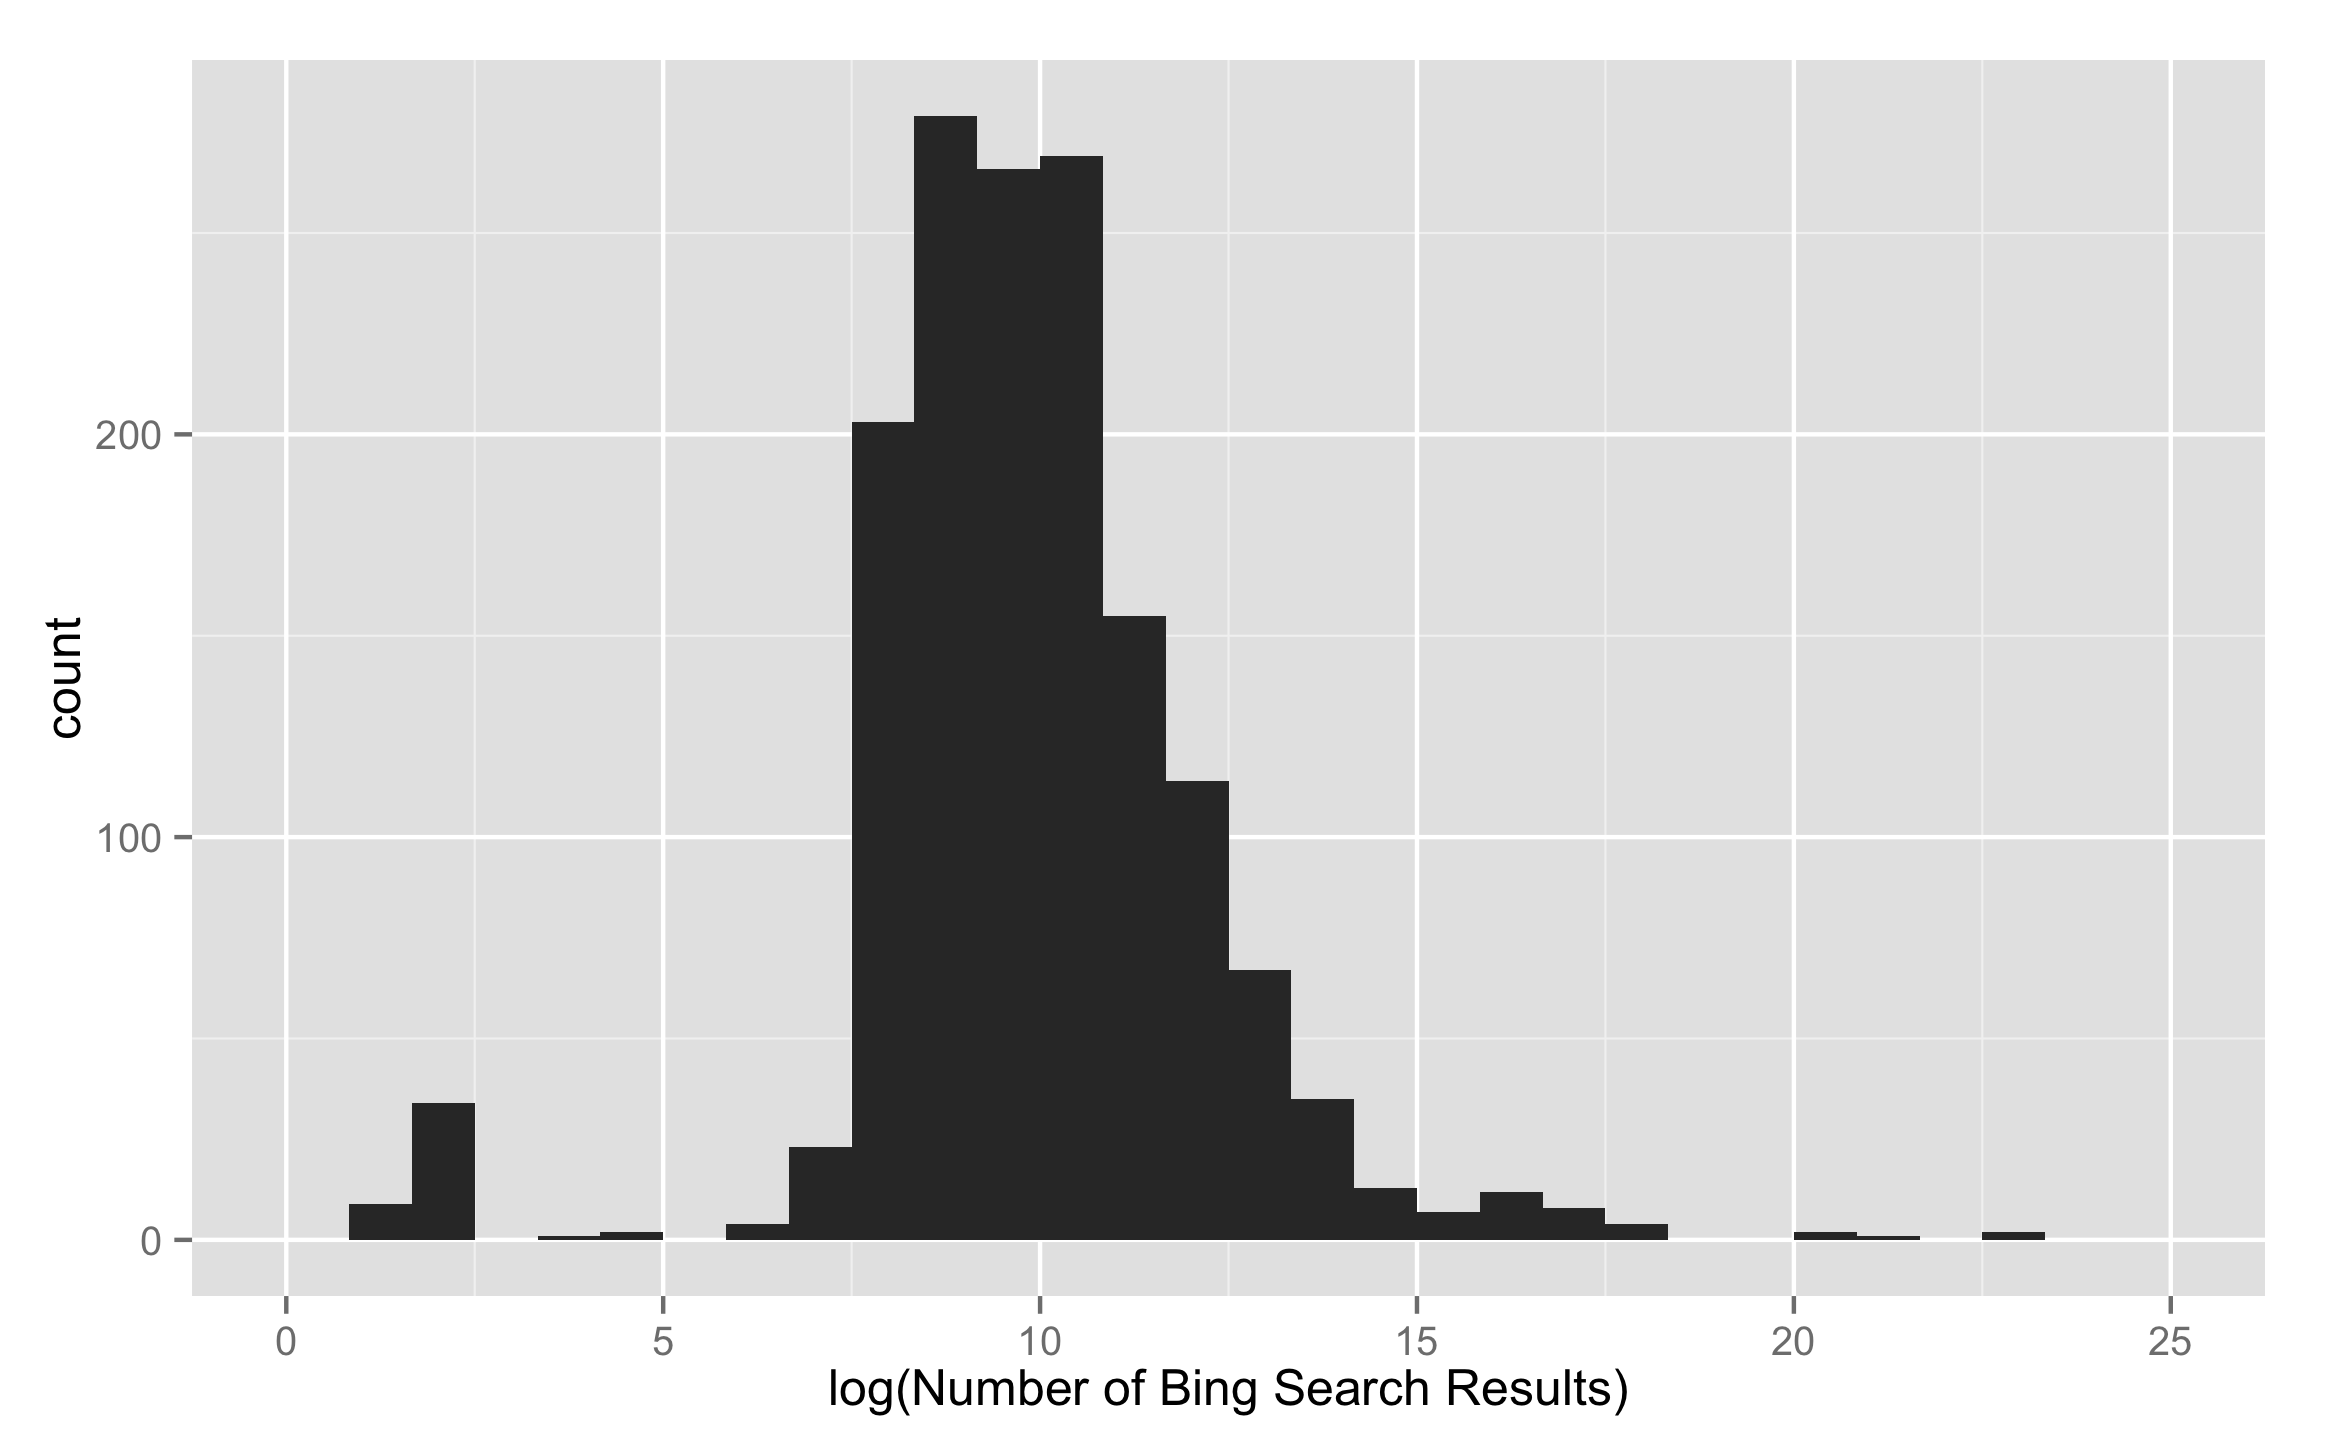
\includegraphics[width=\linewidth]{author_popularity_log_histogram.png}
\caption{Histogram of log(Bing Search Results)}
\label{fig:apl_hist}
\end{figure}
	
\begin{figure}[ht]\centering
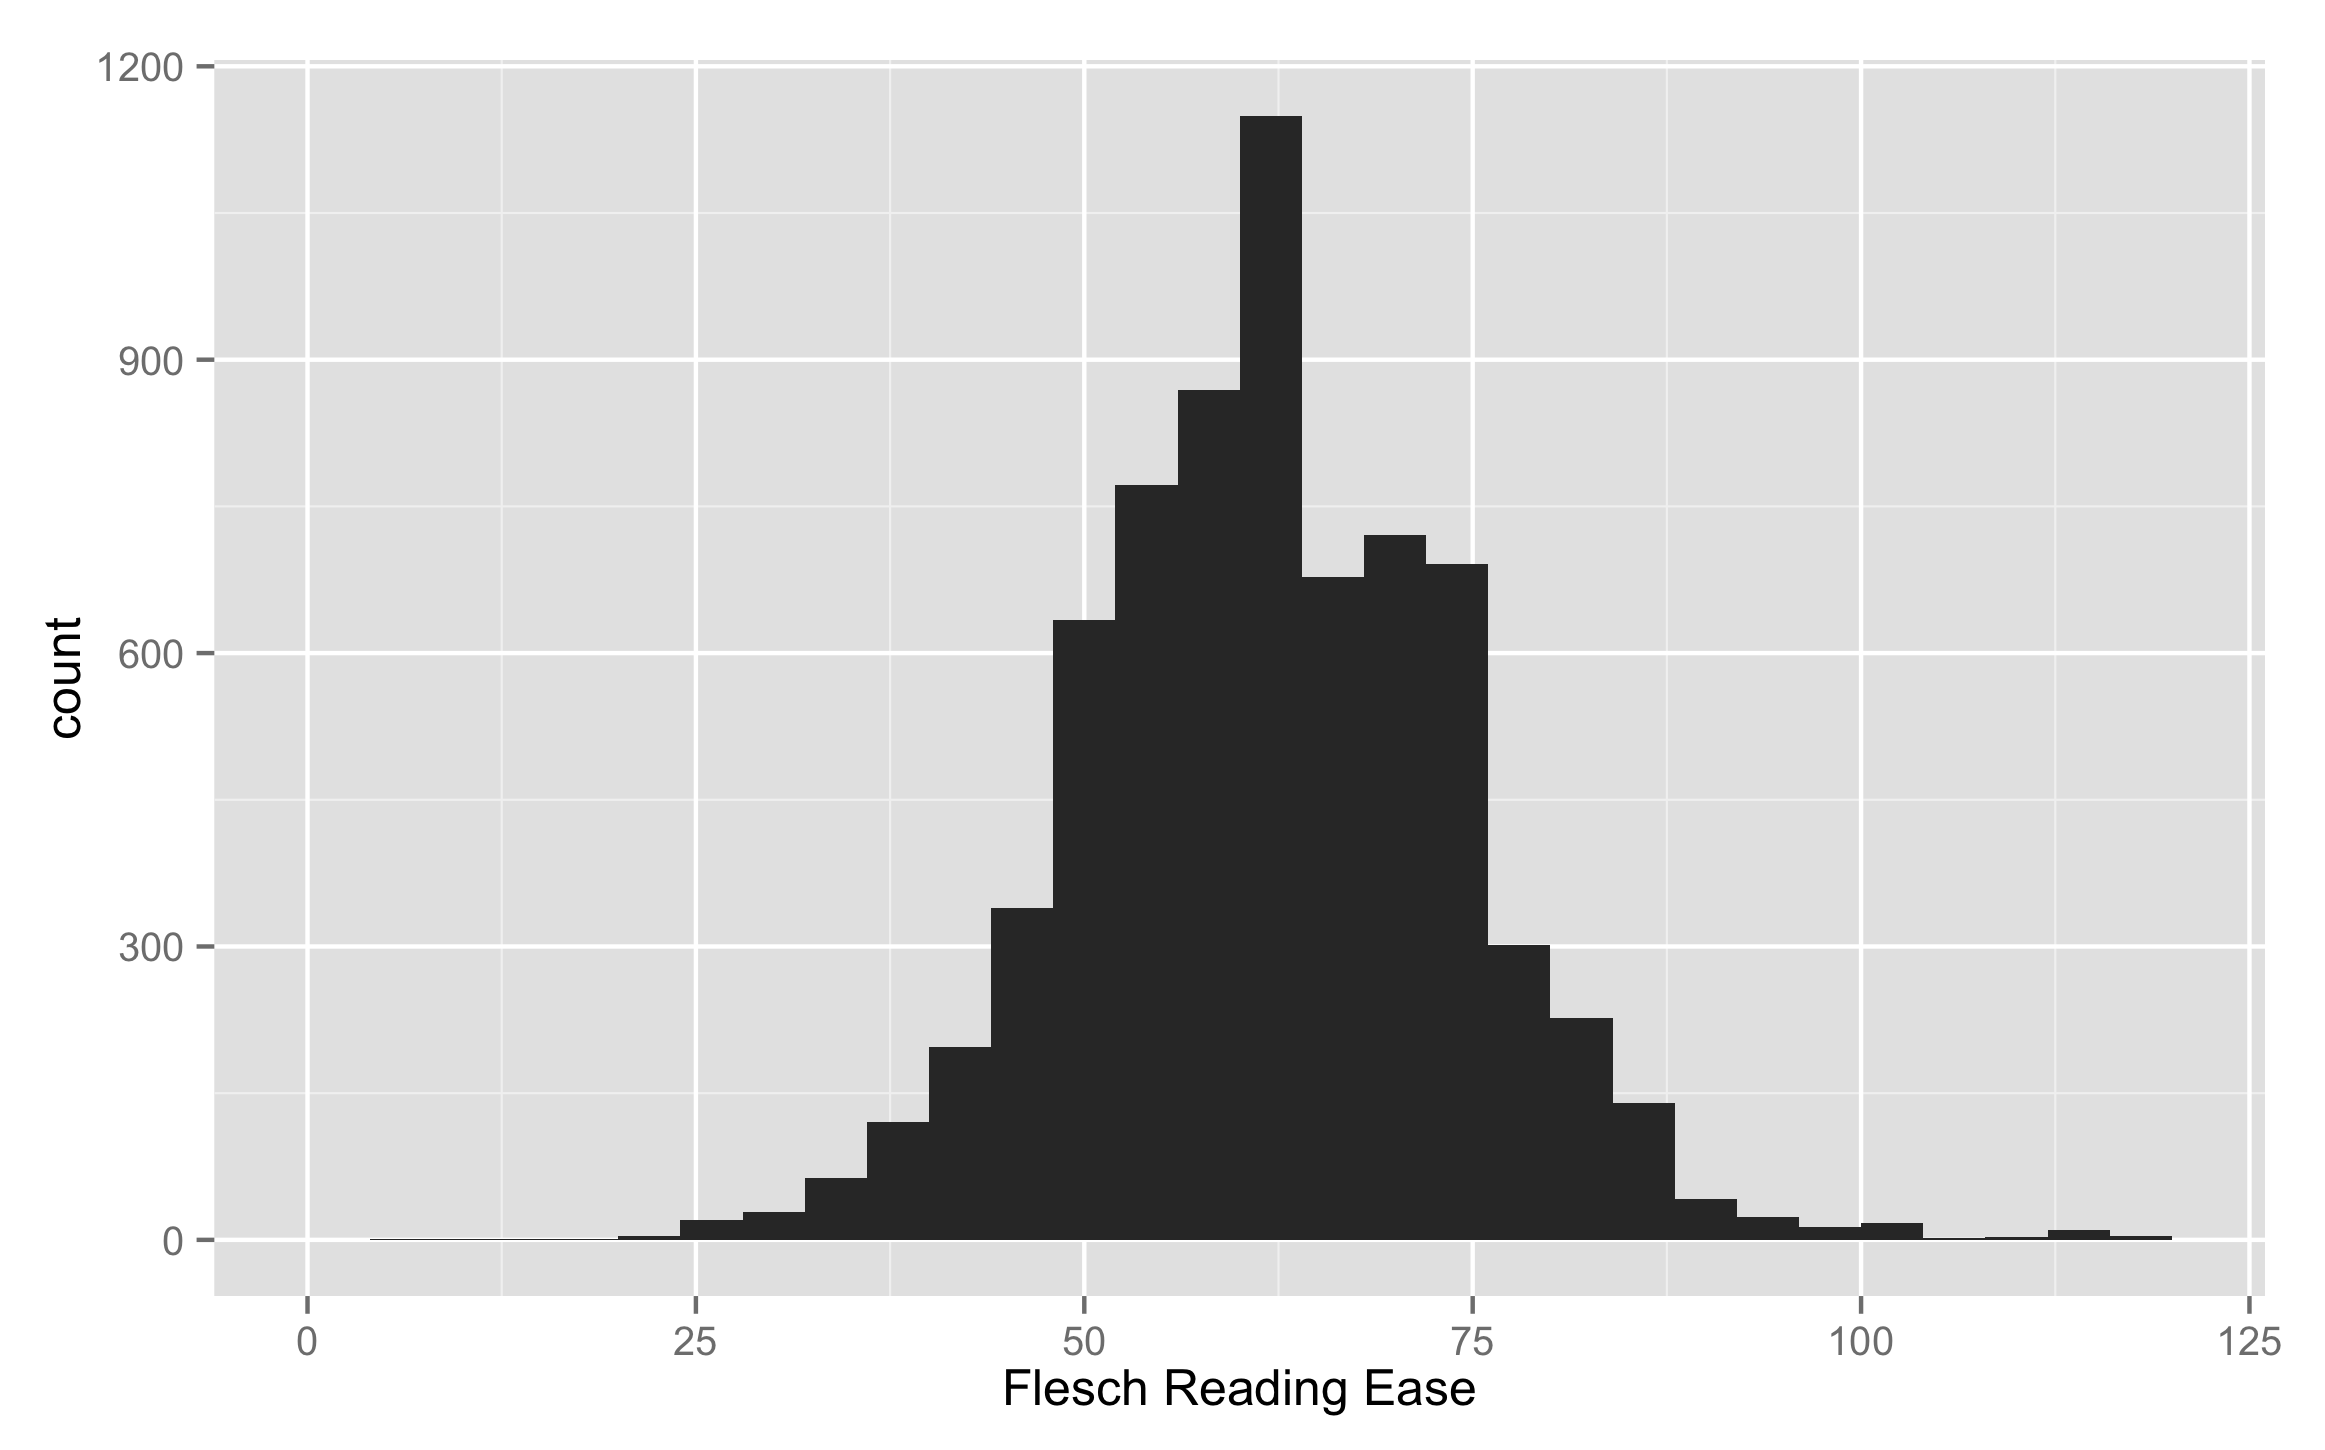
\includegraphics[width=\linewidth]{flesch_data_histogram.png}
\caption{Histogram of Flesch Reading Ease}
\label{fig:fre_hist}
\end{figure}	
	
\end{description}

We also include features that attempt to capture the article sentiment and the article text perplexity. Since the construction of these features was more involved and involved validation of our algorithms, we discuss these two features in separate subsections.

\subsection{Article Sentiment}

\subsection{Article Perplexity}

\section{Predictive Regression Model}

Once we have constructed our full set of features, we aim to predict log(article pageviews), $\mathbf{y}$, using our full set of variables, which we include in our design matrix, $\mathbf{X}$. We estimate the feature weights using the closed form solution for both OLS and ridge regression,

\begin{center}
\begin{equation}
\beta = (\mathbf{X}^T\mathbf{X} + \lambda \mathbf{I})^{-1}\mathbf{X}^T\mathbf{y}
\end{equation}
\end{center}

\noindent where $\mathbf{I}$ is the $k \times k$ identity matrix, and $\lambda$ is our regularization parameter. Setting $\lambda = 0$ corresponds to OLS, whereas non-zero values of $\lambda$ correspond to ridge regression. The motivation for performing ridge regression as opposed to OLS is to not overfit on our data. 

In order to choose an appropriate value of $\lambda$, we split our data into a training and validation set. 90\% of the data is allocated to the training set, and 10\% of the data is allocated to the test set. We cross-validate the estimated $\beta$ values on our validation set for each $\lambda$, and choose the value of $\lambda$ that produces the lowest MSE on the validation data.

The table below displays the 20 feature weights with the largest magnitudes given our model. A bar chart showing the magnitude of all of the weights (excluding the intercept weight) can be found in Figure \ref{fig:lin_reg_weights}.

\begin{figure*}[ht]\centering
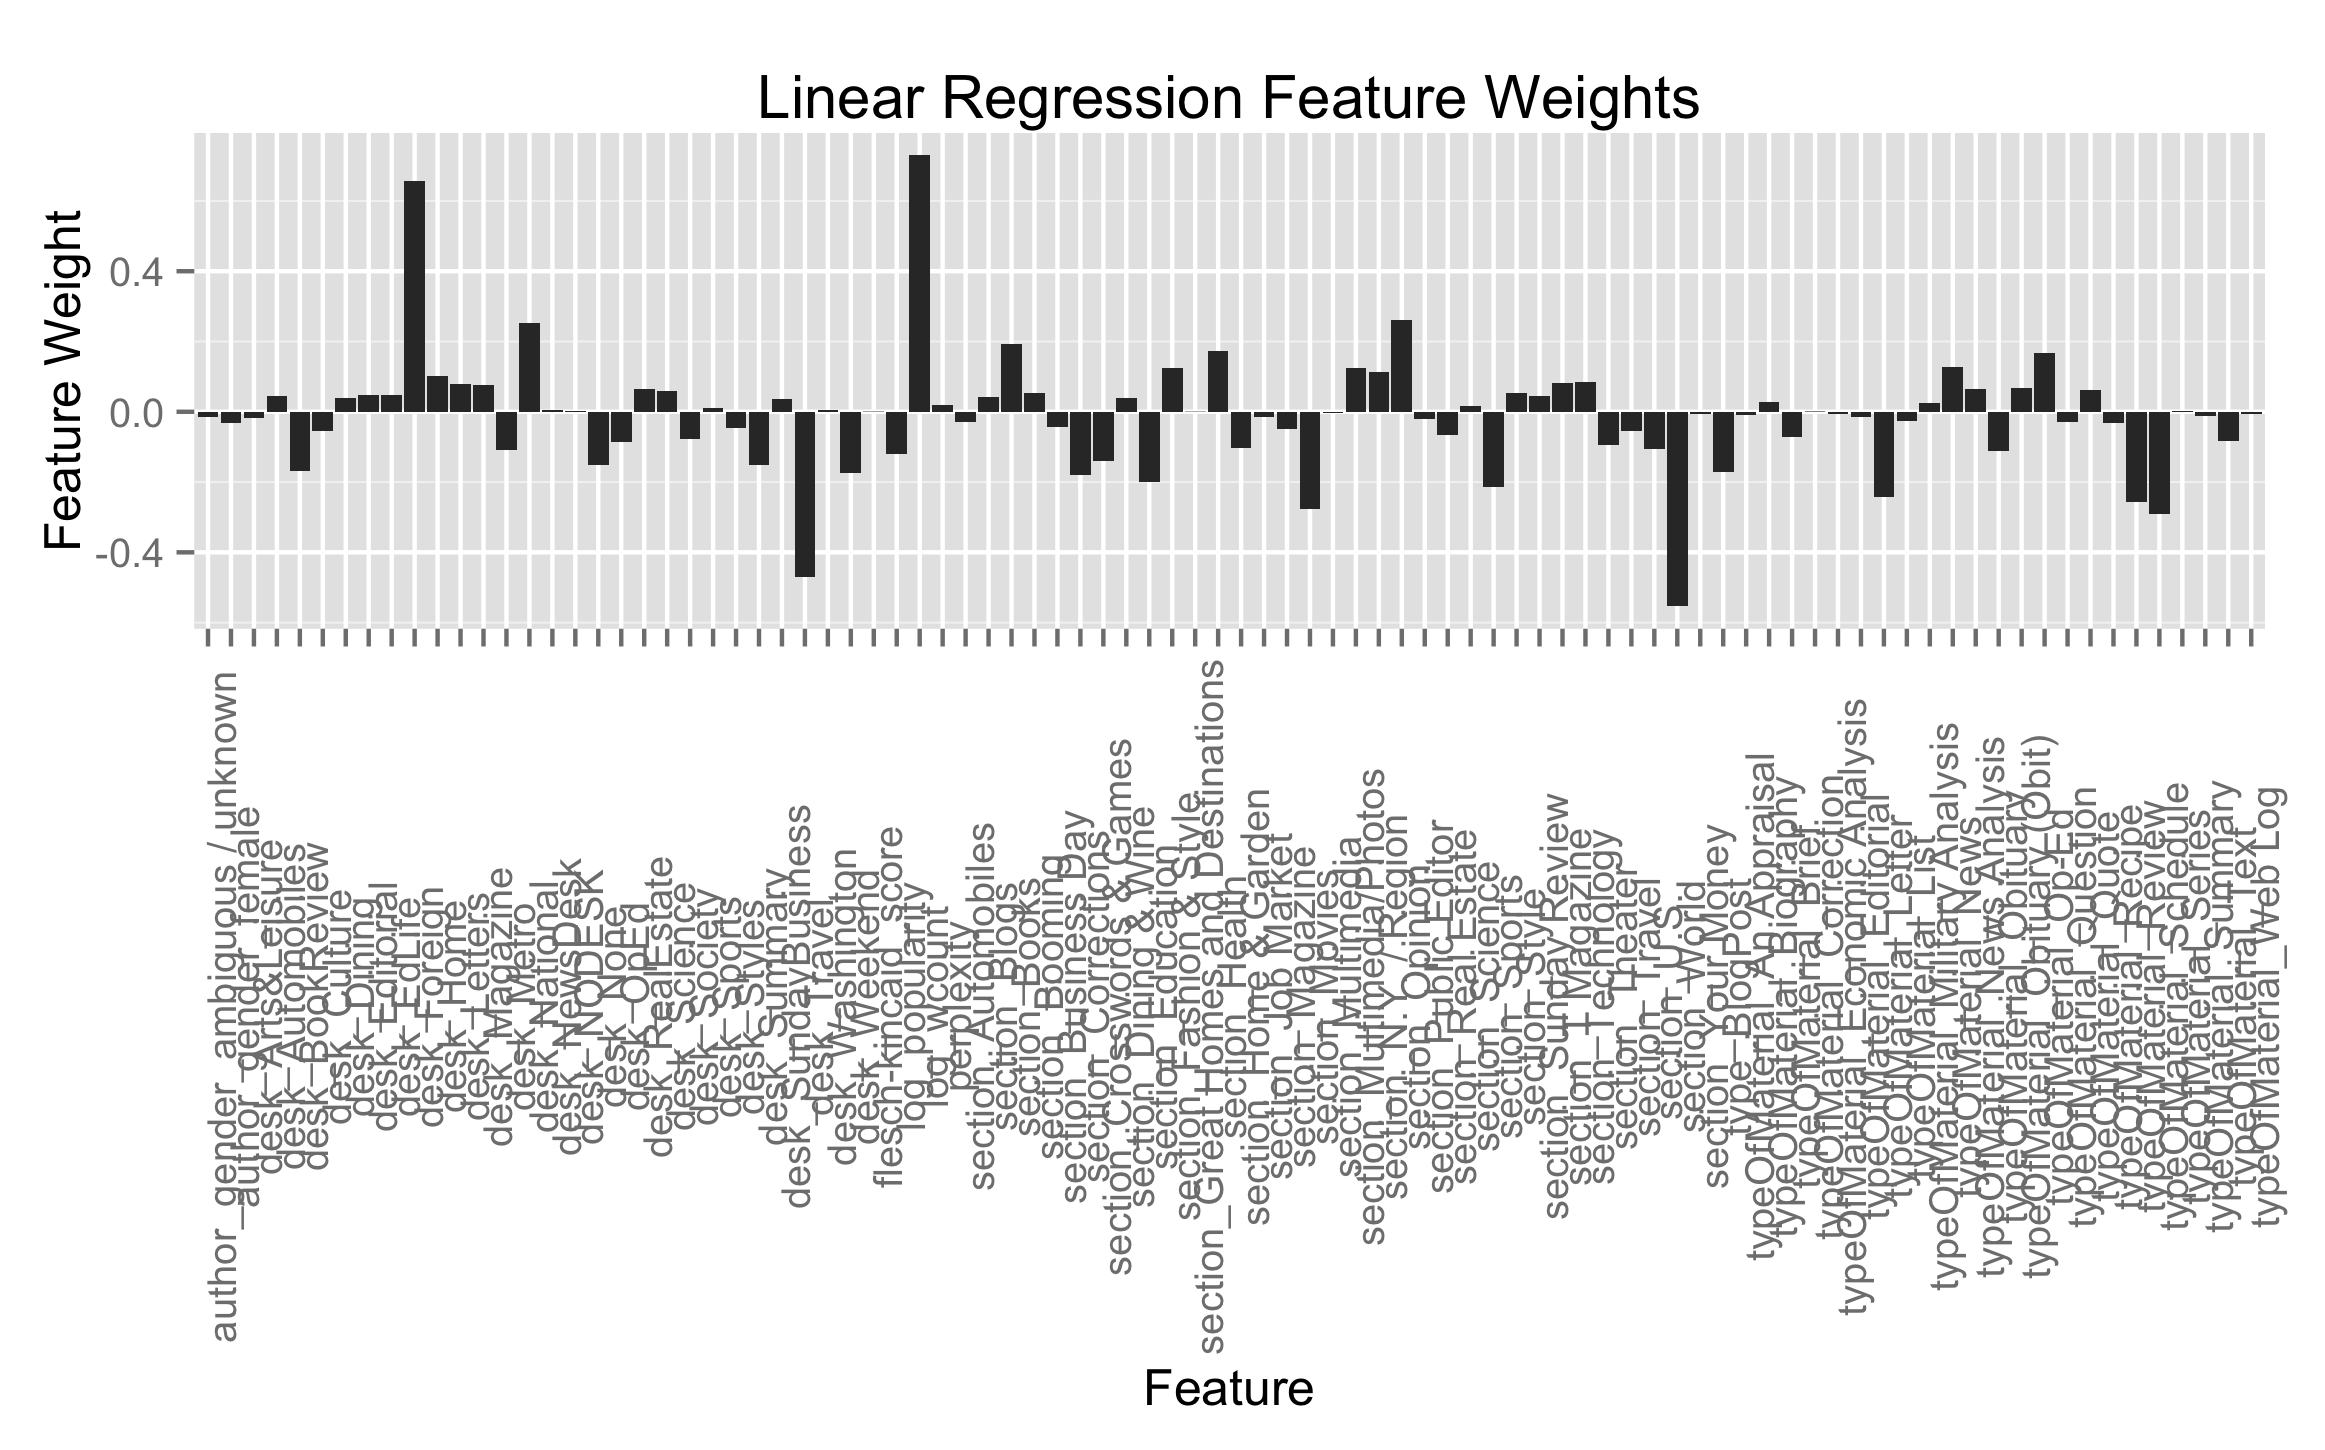
\includegraphics[width=\linewidth]{feature_weights.png}
\caption{Linear Regression Feature Weights (excluding intercept term)}
\label{fig:lin_reg_weights}
\end{figure*}

Figure \ref{fig:mse_plot} shows the training and holdout MSE for various values of Lambda. There are a few things in this plot worth discussing. First, note that the holdout MSE is consistently lower than the training data MSE. Given the (relatively) small size of our dataset (6,687 observations), this is likely due to the sampling we used to separate our data into training and validation data. However, this shouldn't effect the validity of our cross validation.

Another thing worth noting is that even on the training dataset, the MSE goes down once we choose a non-zero value of $\lambda$. At first, this was surprising to our group, as conceptually OLS is often thought of as the linear regression method that minimizes MSE. However, it is important to note that OLS only holds this distinction amongst unbiased estimators. Hoerl and Kennard (1970) \cite{hoerl1970ridge} prove the existence theorem for ridge regression, which proves that there exists a value of $\lambda$ for which $\beta_{ridge}$ produces a lower MSE than $\beta_{OLS}$. 

Another way of framing this finding is through bias-variance tradeoff. Recall that the MSE can be written as a function of the bias and variance:

\begin{equation}
MSE = (\textrm{Bias})^2 + \textrm{Var}.
\end{equation}

\noindent For some values of $\lambda$, ridge regression is able to lower the MSE by decreasing variance, but adding a non-zero bias term. We believe this is what is happening in our data when cycling through different $\lambda$ values.

\begin{figure}[ht]\centering
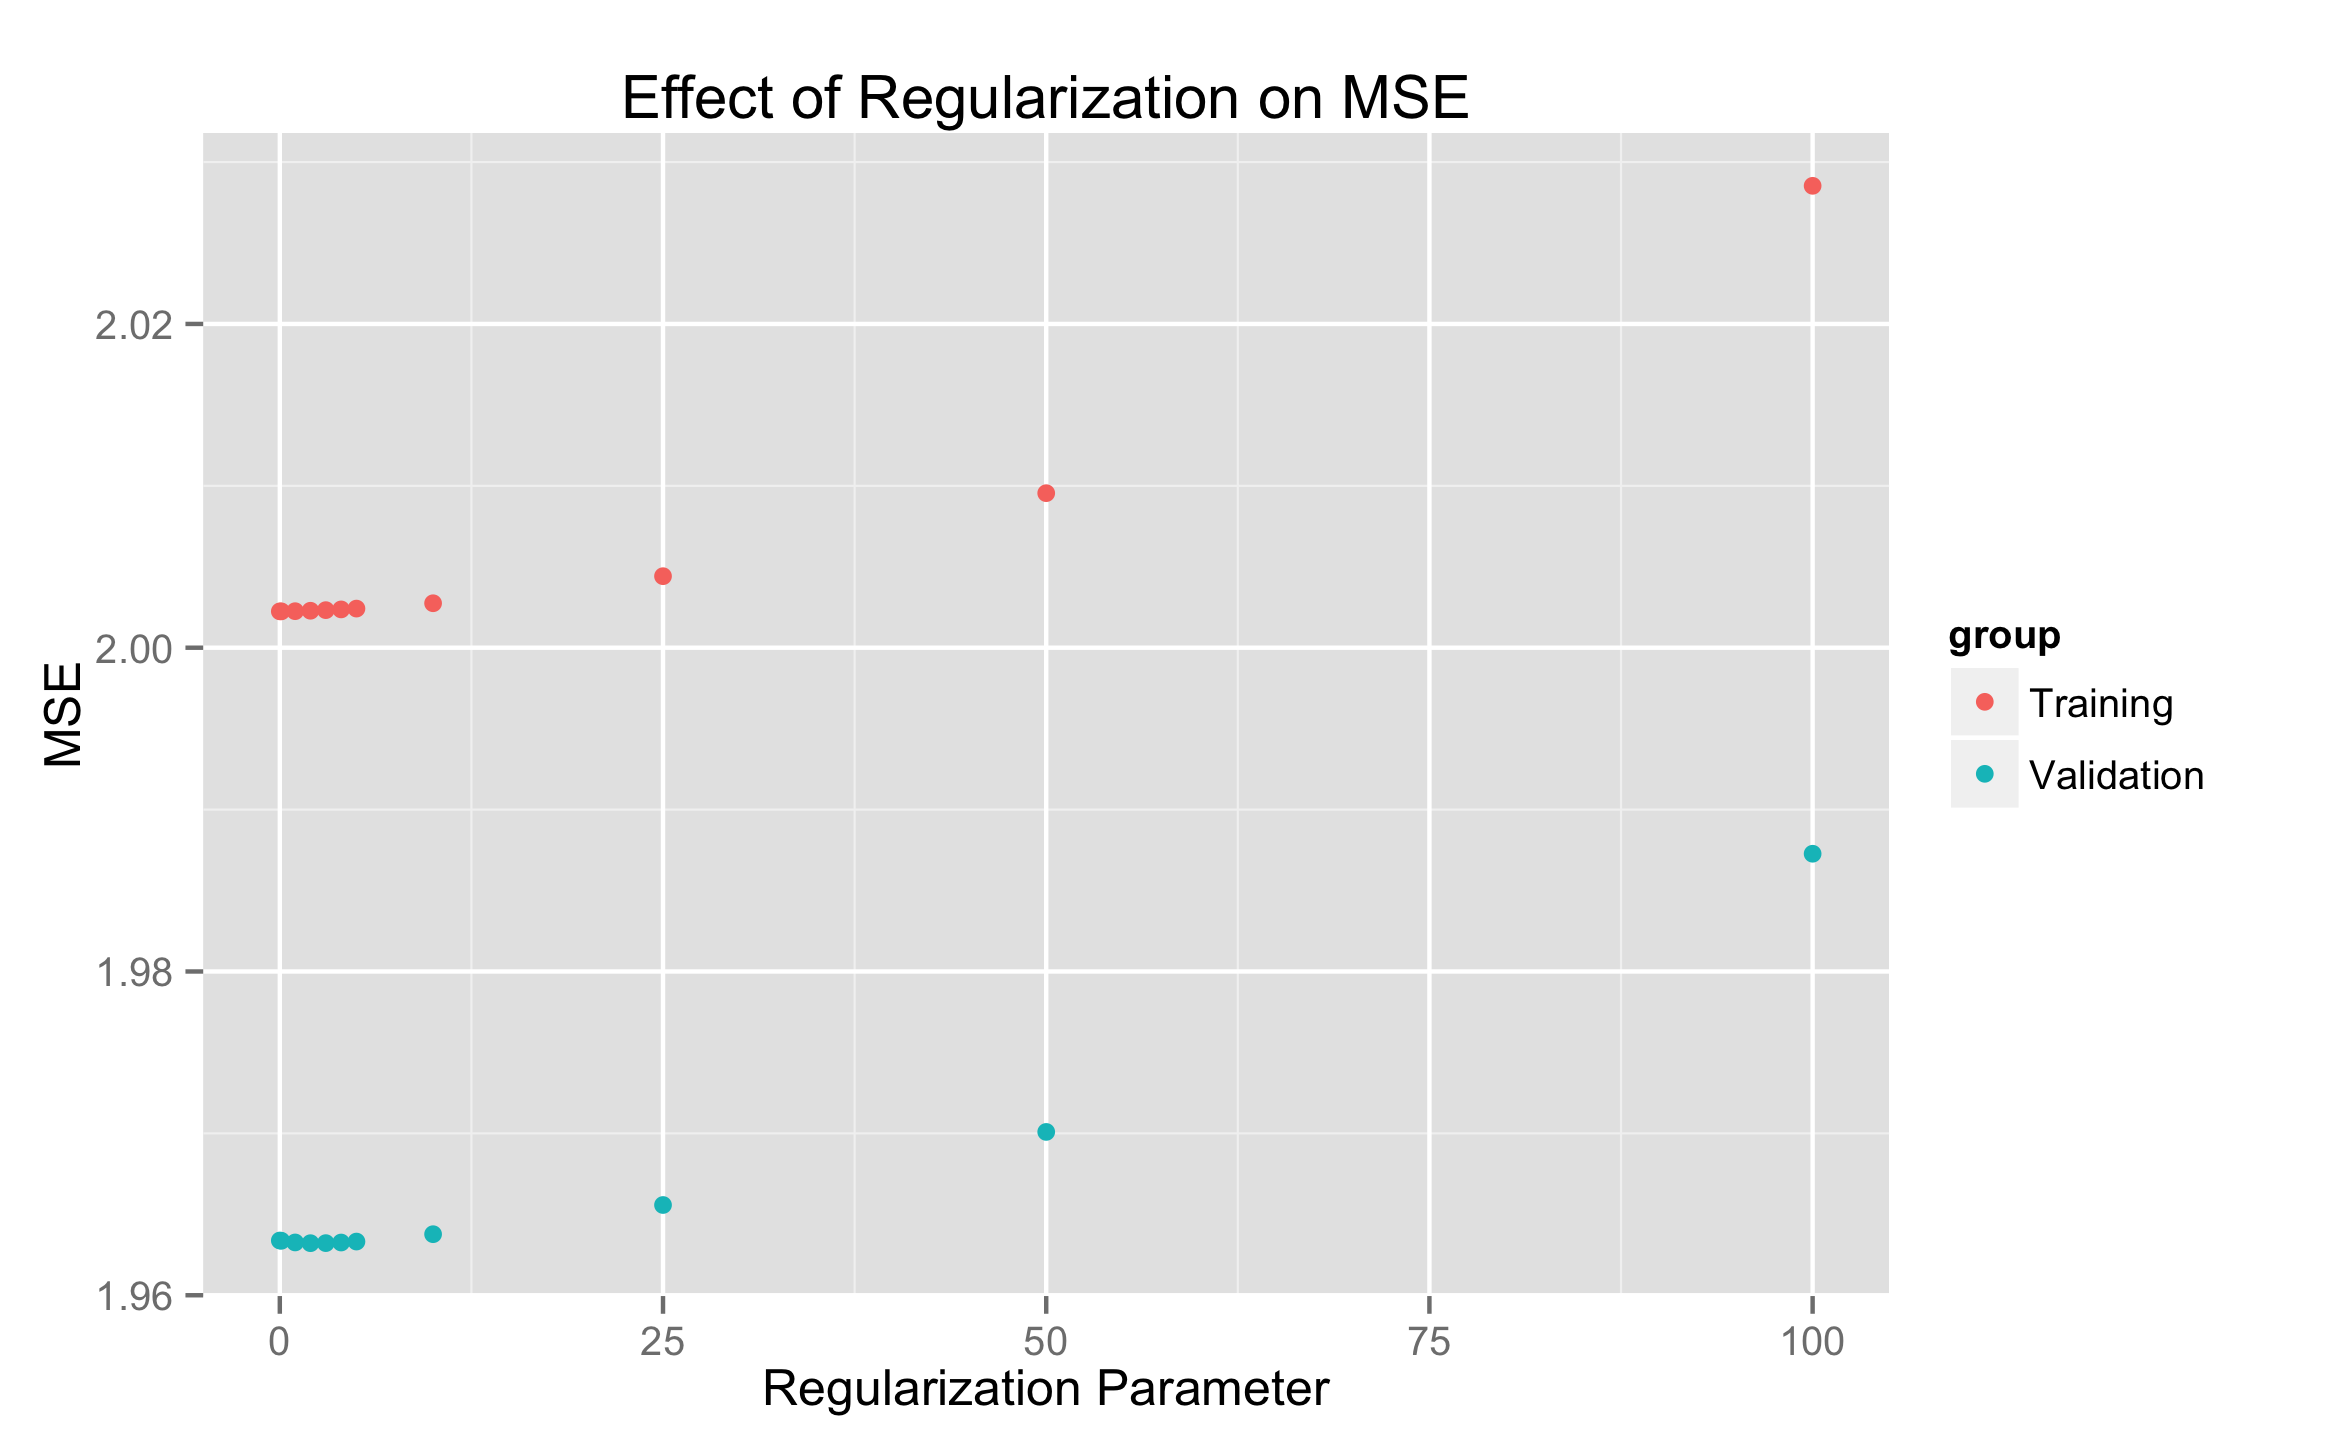
\includegraphics[width=\linewidth]{mse_plot.png}
\caption{The effect of regularization on MSE}
\label{fig:mse_plot}
\end{figure}

\begin{center}
\begin{tabular}{lr}
\toprule
Feature  &  Weight\\
\midrule
intercept & 9.114\\
log(Word Count) & 0.736\\
Desk: Foreign & 0.561\\
Desk: Travel & -0.478\\
Section: World & -0.410\\
Type: BlogPost & -0.394\\
Type of Material: Schedule & -0.330\\
Type of Material: Review & -0.324\\
Type of Material: Letter & -0.311\\
Section: Fashion \& Style & 0.275\\
Section: Movies & -0.267\\
Desk: National & 0.245\\
Section: Opinion & 0.245\\
Time of Day: 12-17 & 0.239\\
Section: Books & 0.219\\
Section: Health & 0.200\\
Section: Sports & -0.191\\
Desk: Society & -0.178\\
Section: Corrections & -0.167\\
Desk: BookReview & -0.167\\
\end{tabular}
\end{center}
%------------------------------------------------
\phantomsection
\section*{Acknowledgments} % The \section*{} command stops section numbering

\addcontentsline{toc}{section}{Acknowledgments} % Adds this section to the table of contents

%----------------------------------------------------------------------------------------
%	REFERENCE LIST
%----------------------------------------------------------------------------------------
\phantomsection
\bibliographystyle{unsrt}
\bibliography{Paper}

%----------------------------------------------------------------------------------------

\end{document}